\newpage
\pagestyle{fancy}
\lhead{\textsc{Chapitre 5. Sprint 3 --- Facturation et tableau de bord}}
\renewcommand{\headrulewidth}{0.5pt}
\renewcommand{\footrulewidth}{0.5pt}
\chapter{Sprint 3 --- Facturation et tableau de bord}\setlength{\headheight}{28pt}
\label{ch5}
\thispagestyle{empty}
\minitoc
\newpage

\section{Introduction}

Suite à l'implémentation des fonctionnalités d'authentification, de gestion du référentiel métier et
de gestion des interventions lors des sprints précédents, ce troisième sprint se concentre sur les
fonctionnalités de supervision et de suivi général du système.

Ce sprint a pour objectif de compléter l'application en y intégrant :

\begin{itemize}
    \item La génération des factures pour les interventions curatives hors contrat ;
    \item Le marquage des factures comme payées ;
    \item L'historique des interventions, différencié par rôle ;
    \item Les tableaux de bord différenciés (administrateur, technicien, client).
\end{itemize}

% ─────────────────────────────────────────────────────────────────────────────
\section{Backlog du Sprint 3}

\begin{longtable}{|p{1.2cm}|p{7.5cm}|p{2.8cm}|p{1.8cm}|}
\caption{Backlog du Sprint 3}
\label{tab:ch5:backlog_sprint3} \\
\hline
\textbf{ID} & \textbf{User Story} & \textbf{Acteur} & \textbf{Priorité} \\
\hline
\endfirsthead
\caption*{Backlog du Sprint 3 (suite)} \\
\hline
\textbf{ID} & \textbf{User Story} & \textbf{Acteur} & \textbf{Priorité} \\
\hline
\endhead
\hline
\endfoot
\hline
\endlastfoot
US-19 & En tant qu'administrateur, je veux générer une facture pour une intervention curative réalisée hors contrat (TVA 19\,\%, TND). & Administrateur & Élevée \\
\hline
US-20 & En tant qu'administrateur, je veux marquer une facture comme payée. & Administrateur & Élevée \\
\hline
US-21 & En tant qu'administrateur, je veux consulter toutes les factures avec filtres (statut, client, date). & Administrateur & Élevée \\
\hline
US-24 & En tant que client, je veux consulter l'historique des interventions sur mes équipements. & Client & Moyenne \\
\hline
US-25 & En tant qu'administrateur, je veux consulter un tableau de bord global avec KPIs et graphiques. & Administrateur & Élevée \\
\hline
US-26 & En tant que technicien, je veux consulter mon tableau de bord personnel. & Technicien & Élevée \\
\hline
US-27 & En tant que client, je veux consulter mon espace personnel. & Client & Élevée \\
\hline
\end{longtable}

% ─────────────────────────────────────────────────────────────────────────────
\section{Analyse}

\subsection{Diagramme de cas d'utilisation du Sprint 3}

\begin{figure}[H]
\centering
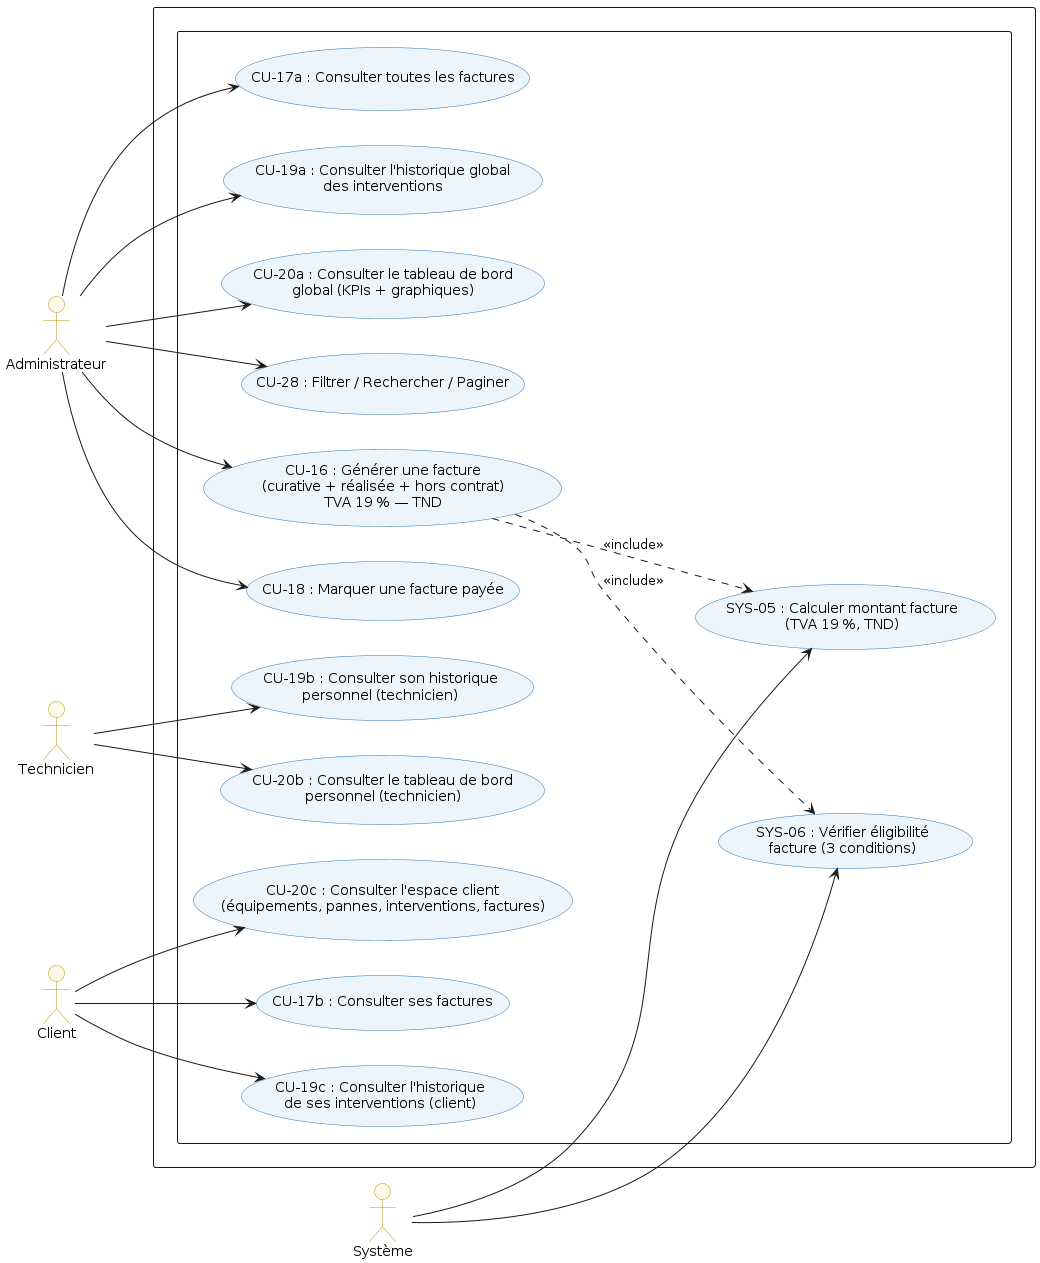
\includegraphics[width=0.70\textwidth]{Figures/Chapitre5/use_case_sprint3.png}
\caption{Diagramme de cas d'utilisation du Sprint 3}
\label{fig:ch5:use_case_sprint3}
\end{figure}

Les acteurs impliqués dans ce sprint sont :

\textbf{Administrateur} : génération et consultation des factures, marquage payée, historique global,
tableau de bord administrateur.

\textbf{Technicien} : consultation de son historique, consultation de son tableau de bord personnel.

\textbf{Client} : consultation de ses factures, de son historique, de son espace personnel.

\subsection{Description des cas d'utilisation}

\subsubsection{CU-16 : Générer une facture}

\begin{table}[H]
\centering
\caption{CU-16 : Générer une facture}
\label{tab:ch5:cu16}
\begin{tabular}{|p{3.5cm}|p{11cm}|}
\hline
\textbf{Champ} & \textbf{Contenu} \\
\hline
Description & Ce cas d'utilisation permet à l'administrateur de générer une facture pour une
intervention éligible. \\
\hline
Acteur principal & Administrateur \\
\hline
Préconditions & L'administrateur est authentifié ; une intervention curative réalisée et hors
couverture contractuelle existe. \\
\hline
Postconditions & La facture est créée et enregistrée dans la base de données. \\
\hline
\end{tabular}
\end{table}

\textbf{Règles d'éligibilité (trois conditions cumulatives) :}

\begin{itemize}
    \item Type de l'intervention = \texttt{CURATIVE}
    \item Statut de l'intervention = \texttt{REALISEE}
    \item Couverture contractuelle = false (\texttt{couvertureContrat} = false)
\end{itemize}

\textbf{Scénario nominal :}

\begin{enumerate}
    \item L'administrateur accède à la liste des interventions éligibles à la facturation.
    \item Il sélectionne une intervention répondant aux trois conditions.
    \item Il saisit les lignes de détail de la facture (\texttt{LigneFacture}) : main-d'œuvre et matériel utilisé.
    \item L'Interface transmet les données au Contrôleur.
    \item Le Contrôleur vérifie les trois conditions d'éligibilité.
    \item Le Contrôleur calcule le montant HT (somme des lignes), la TVA (19\,\%) et le montant TTC.
    \item La base de données enregistre la facture et ses lignes de détail.
    \item La base confirme la création.
    \item L'Interface affiche la facture générée.
\end{enumerate}

\textbf{Règles de gestion :}

\begin{itemize}
    \item \textbf{Les interventions préventives ne génèrent jamais de facture.}
    \item \textbf{Les interventions curatives couvertes par un contrat actif ne génèrent pas de facture.}
    \item La TVA est de \textbf{19\,\%} : \texttt{montantTTC} = \texttt{montantHT} $\times$ 1,19.
    \item La monnaie est le \textbf{Dinar Tunisien (TND)}.
    \item La facture est créée avec le statut \texttt{IMPAYEE} ou \texttt{EN\_ATTENTE}.
\end{itemize}

\textit{Mise à jour du statut de paiement :} Après génération, l'administrateur peut mettre à jour l'état de paiement de la facture (passage au statut \texttt{PAYEE}).

\subsubsection{CU-17 : Consulter les factures}

\begin{table}[H]
\centering
\caption{CU-17 : Consulter les factures}
\label{tab:ch5:cu17}
\begin{tabular}{|p{3.5cm}|p{11cm}|}
\hline
\textbf{Champ} & \textbf{Contenu} \\
\hline
Description & Ce cas d'utilisation permet de consulter les factures selon les droits d'accès. \\
\hline
Acteurs & Administrateur, Client \\
\hline
Préconditions & L'utilisateur est authentifié. \\
\hline
Postconditions & Les factures accessibles à l'utilisateur sont affichées en lecture seule. \\
\hline
\end{tabular}
\end{table}

\textbf{Scénario nominal :} L'utilisateur accède au module des factures ; le système filtre selon le rôle (toutes pour l'administrateur, uniquement les siennes pour le client) et affiche les résultats avec les filtres disponibles.

\textbf{Règles de gestion :}

\begin{itemize}
    \item Le client ne peut consulter que ses propres factures.
    \item La consultation est en lecture seule pour le client.
    \item L'administrateur peut appliquer des filtres par statut, client et date d'émission.
\end{itemize}

\subsubsection{CU-19 : Consulter le tableau de bord administrateur}

\begin{table}[H]
\centering
\caption{CU-19 : Consulter le tableau de bord administrateur}
\label{tab:ch5:cu19}
\begin{tabular}{|p{3.5cm}|p{11cm}|}
\hline
\textbf{Champ} & \textbf{Contenu} \\
\hline
Description & Permet à l'administrateur de consulter les indicateurs globaux du système SAV. \\
\hline
Acteur principal & Administrateur \\
\hline
Préconditions & L'administrateur est authentifié ; des données existent dans le système. \\
\hline
Postconditions & Les statistiques et graphiques sont affichés. \\
\hline
\end{tabular}
\end{table}

\textbf{Contenu du tableau de bord :} KPIs globaux (interventions, contrats, clients, équipements), chiffre d'affaires mensuel, factures impayées, graphiques d'activité mensuelle et répartition préventif/curatif.

\subsubsection{CU-20 : Consulter le tableau de bord technicien}

\begin{table}[H]
\centering
\caption{CU-20 : Consulter le tableau de bord technicien}
\label{tab:ch5:cu20}
\begin{tabular}{|p{3.5cm}|p{11cm}|}
\hline
\textbf{Champ} & \textbf{Contenu} \\
\hline
Description & Permet au technicien de consulter son tableau de bord personnel. \\
\hline
Acteur principal & Technicien \\
\hline
Préconditions & Le technicien est authentifié. \\
\hline
Postconditions & Les indicateurs personnels et le planning du technicien sont affichés. \\
\hline
\end{tabular}
\end{table}

\textbf{Contenu du tableau de bord :} Nombre d'interventions assignées, taux de réalisation, planning de la semaine en cours et dernières interventions réalisées.

\subsubsection{CU-21 : Consulter l'espace client}

\begin{table}[H]
\centering
\caption{CU-21 : Consulter l'espace client (dashboard client)}
\label{tab:ch5:cu21}
\begin{tabular}{|p{3.5cm}|p{11cm}|}
\hline
\textbf{Champ} & \textbf{Contenu} \\
\hline
Description & Permet au client de consulter un résumé de sa situation dans le système. \\
\hline
Acteur principal & Client \\
\hline
Préconditions & Le client est authentifié. \\
\hline
Postconditions & L'espace personnel du client est affiché. \\
\hline
\end{tabular}
\end{table}

\textbf{Contenu de l'espace client :} Équipements affectés, interventions en cours, pannes ouvertes et factures en attente de paiement.

\subsubsection{CU-22 : Consulter l'historique des interventions}

\begin{table}[H]
\centering
\caption{CU-22 : Consulter l'historique des interventions}
\label{tab:ch5:cu22}
\begin{tabular}{|p{3.5cm}|p{11cm}|}
\hline
\textbf{Champ} & \textbf{Contenu} \\
\hline
Description & Permet de consulter l'historique des interventions réalisées ou annulées, filtré selon le rôle. \\
\hline
Acteurs & Administrateur, Technicien, Client \\
\hline
Préconditions & L'utilisateur est authentifié. \\
\hline
Postconditions & L'historique filtré selon le rôle est affiché. \\
\hline
\end{tabular}
\end{table}

\textbf{Scénario nominal :}

\begin{enumerate}
    \item L'utilisateur ouvre le module Historique.
    \item Le Contrôleur filtre les interventions selon le rôle :
    \begin{itemize}
        \item Administrateur $\rightarrow$ toutes les interventions avec statut \texttt{REALISEE} ou \texttt{ANNULEE}.
        \item Technicien $\rightarrow$ uniquement ses interventions assignées avec ces statuts.
        \item Client $\rightarrow$ uniquement les interventions liées à ses \texttt{ClientEquipement}.
    \end{itemize}
    \item Les résultats sont affichés avec filtres (date, type, statut, client, technicien selon le rôle).
\end{enumerate}

Des filtres permettent de faciliter la consultation de l'historique et des tableaux de bord.

% ─────────────────────────────────────────────────────────────────────────────
\section{Conception}

\subsection{Diagramme de classes du Sprint 3}

\begin{figure}[H]
\centering
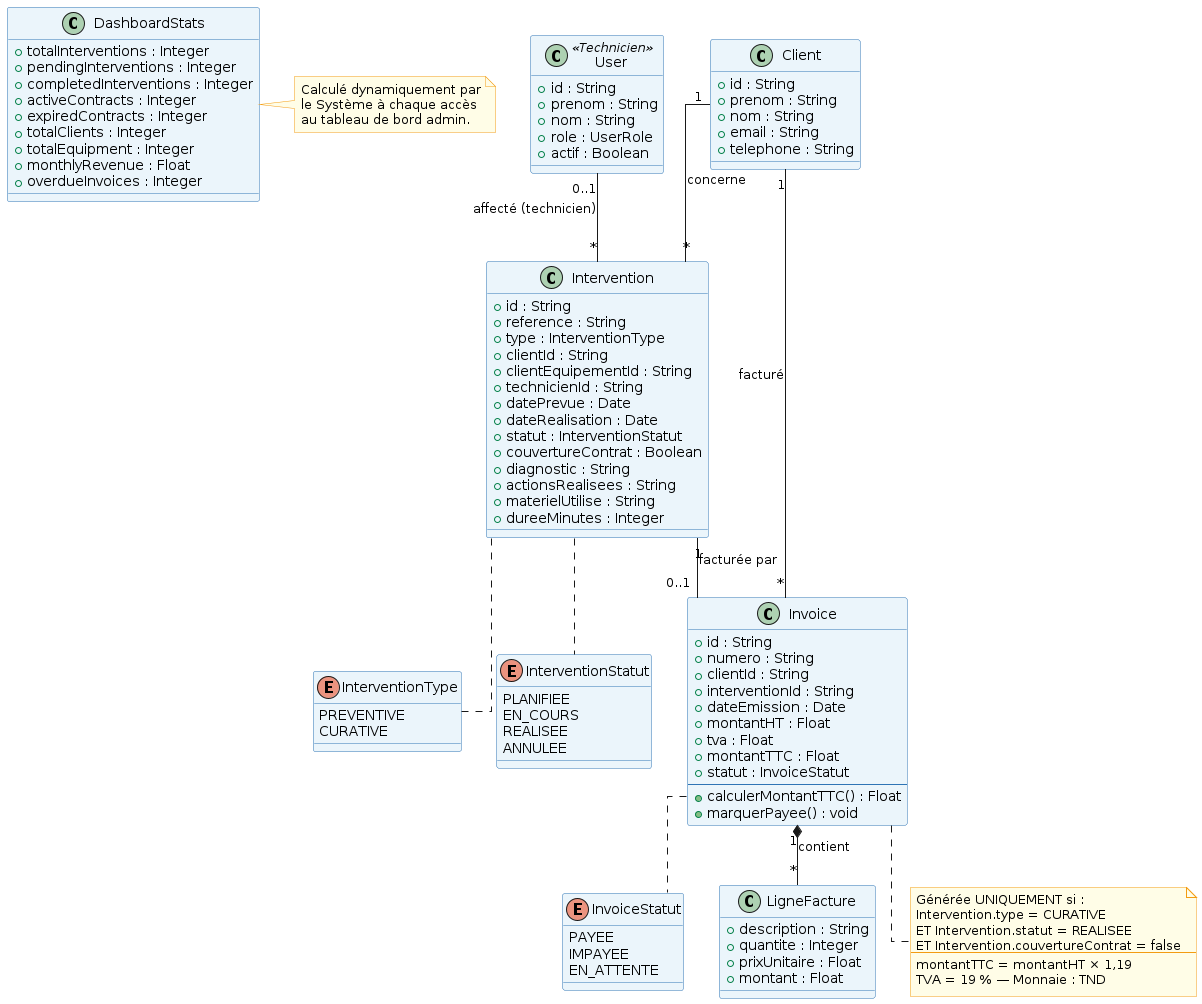
\includegraphics[width=0.70\textwidth]{Figures/Chapitre5/class_diagram_sprint3.png}
\caption{Diagramme de classes du Sprint 3}
\label{fig:ch5:class_sprint3}
\end{figure}

Les entités impliquées dans ce sprint sont : \texttt{Facture}, \texttt{LigneFacture},
\texttt{Intervention}, \texttt{Contract}, Client, User.

\subsection{Diagrammes de séquence}

\subsubsection{Diagramme de séquence : Génération d'une facture}

\begin{figure}[H]
\centering
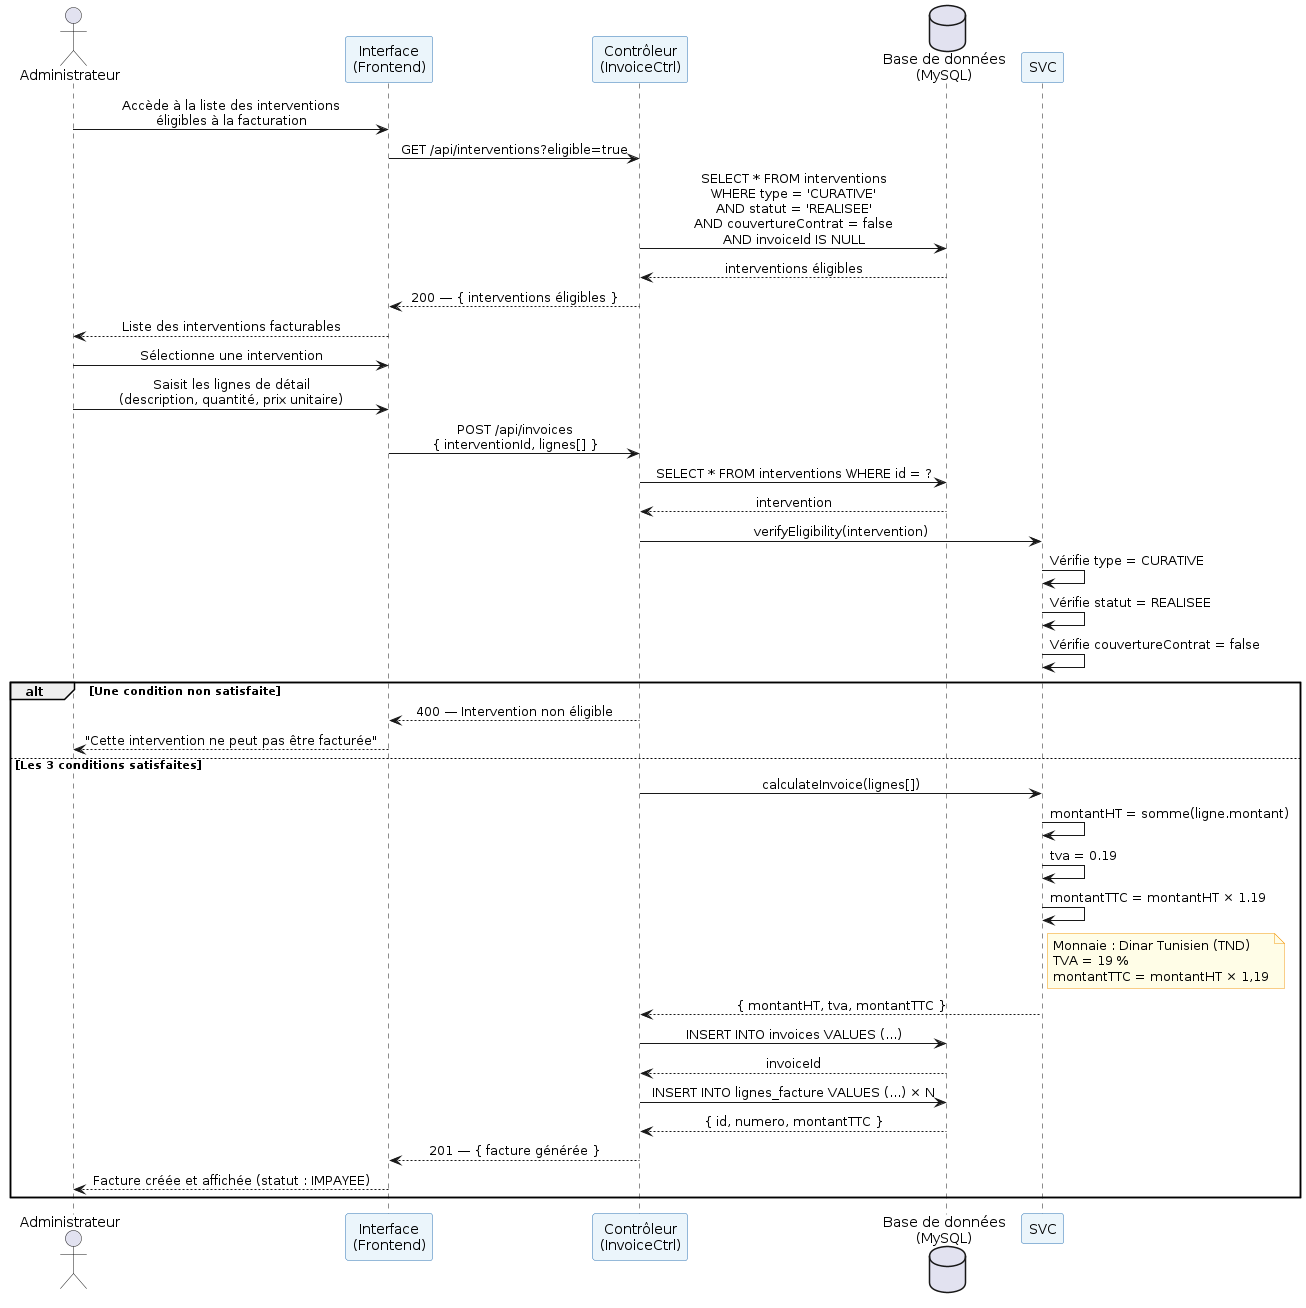
\includegraphics[width=0.70\textwidth]{Figures/Chapitre5/seq_genererfacture_sprint3.png}
\caption{Diagramme de séquence : Génération d'une facture}
\label{fig:ch5:seq_generation_facture}
\end{figure}
\subsubsection{Diagramme de séquence : Consultation de l'historique côté client}

\begin{figure}[H]
\centering
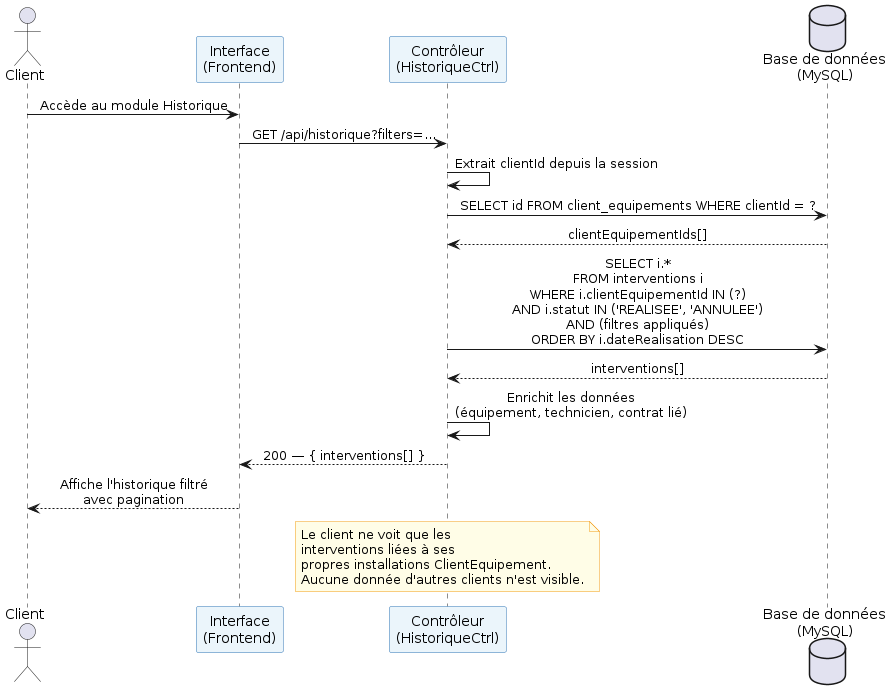
\includegraphics[width=0.70\textwidth]{Figures/Chapitre5/seq_historiqueclient_sprint3.png}
\caption{Diagramme de séquence : Consultation de l'historique côté client}
\label{fig:ch5:seq_historique_client}
\end{figure}

% ─────────────────────────────────────────────────────────────────────────────
\section{Réalisation}

\begin{figure}[H]
\centering
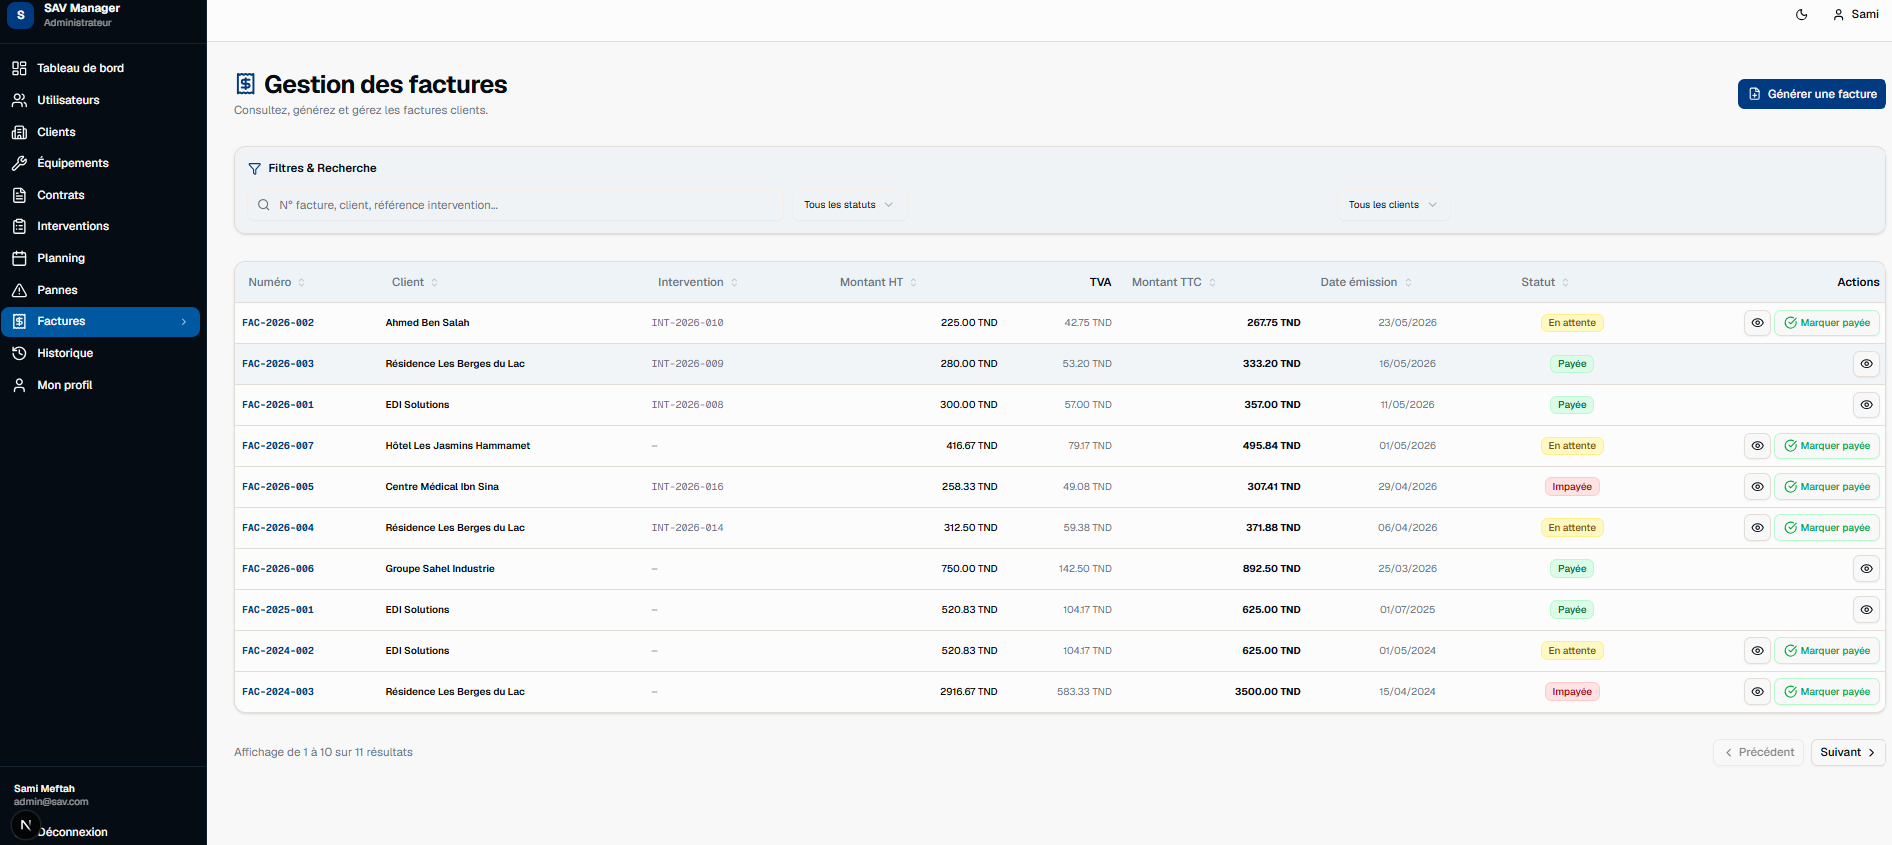
\includegraphics[width=0.65\textwidth]{Figures/Chapitre5/gestfacture.png}
\caption{Capture d'écran de la gestion des factures}
\label{fig:ch4:gestion_factures}
\end{figure}

\begin{figure}[H]
    \centering
    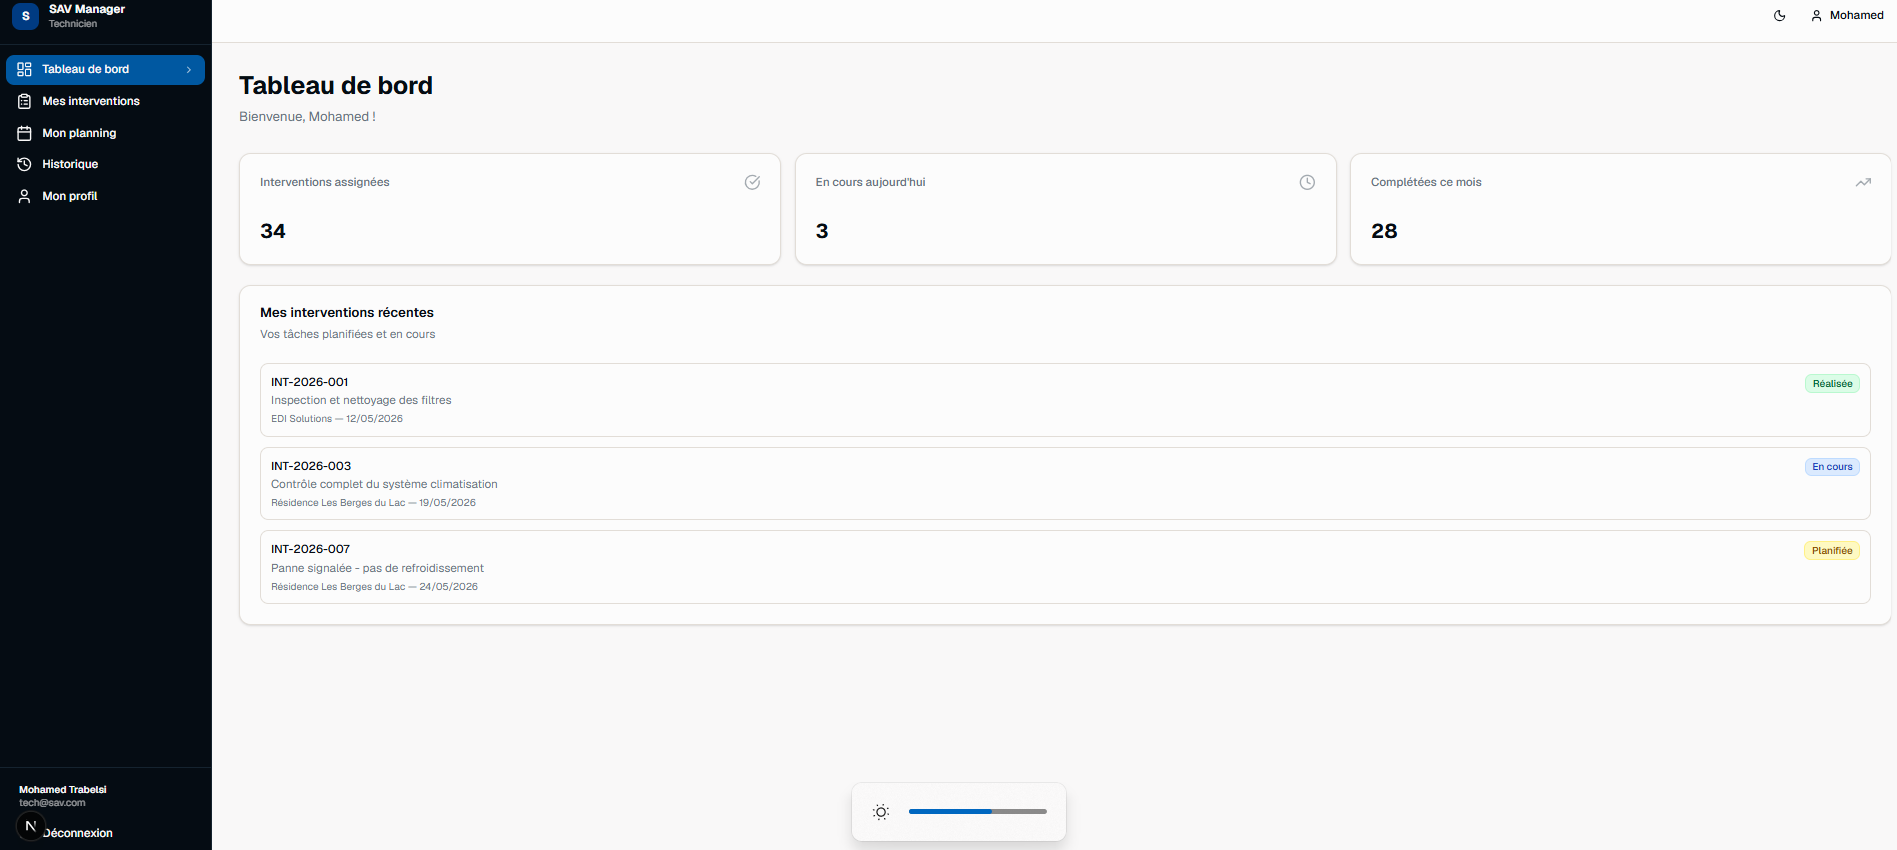
\includegraphics[width=0.74\textwidth]{Figures/Chapitre5/dashboardtech.png}
    \caption{Capture d'écran : tableau de bord technicien}
    \label{fig:ch5:dashboard_technicien}
\end{figure}

\begin{figure}[H]
    \centering
    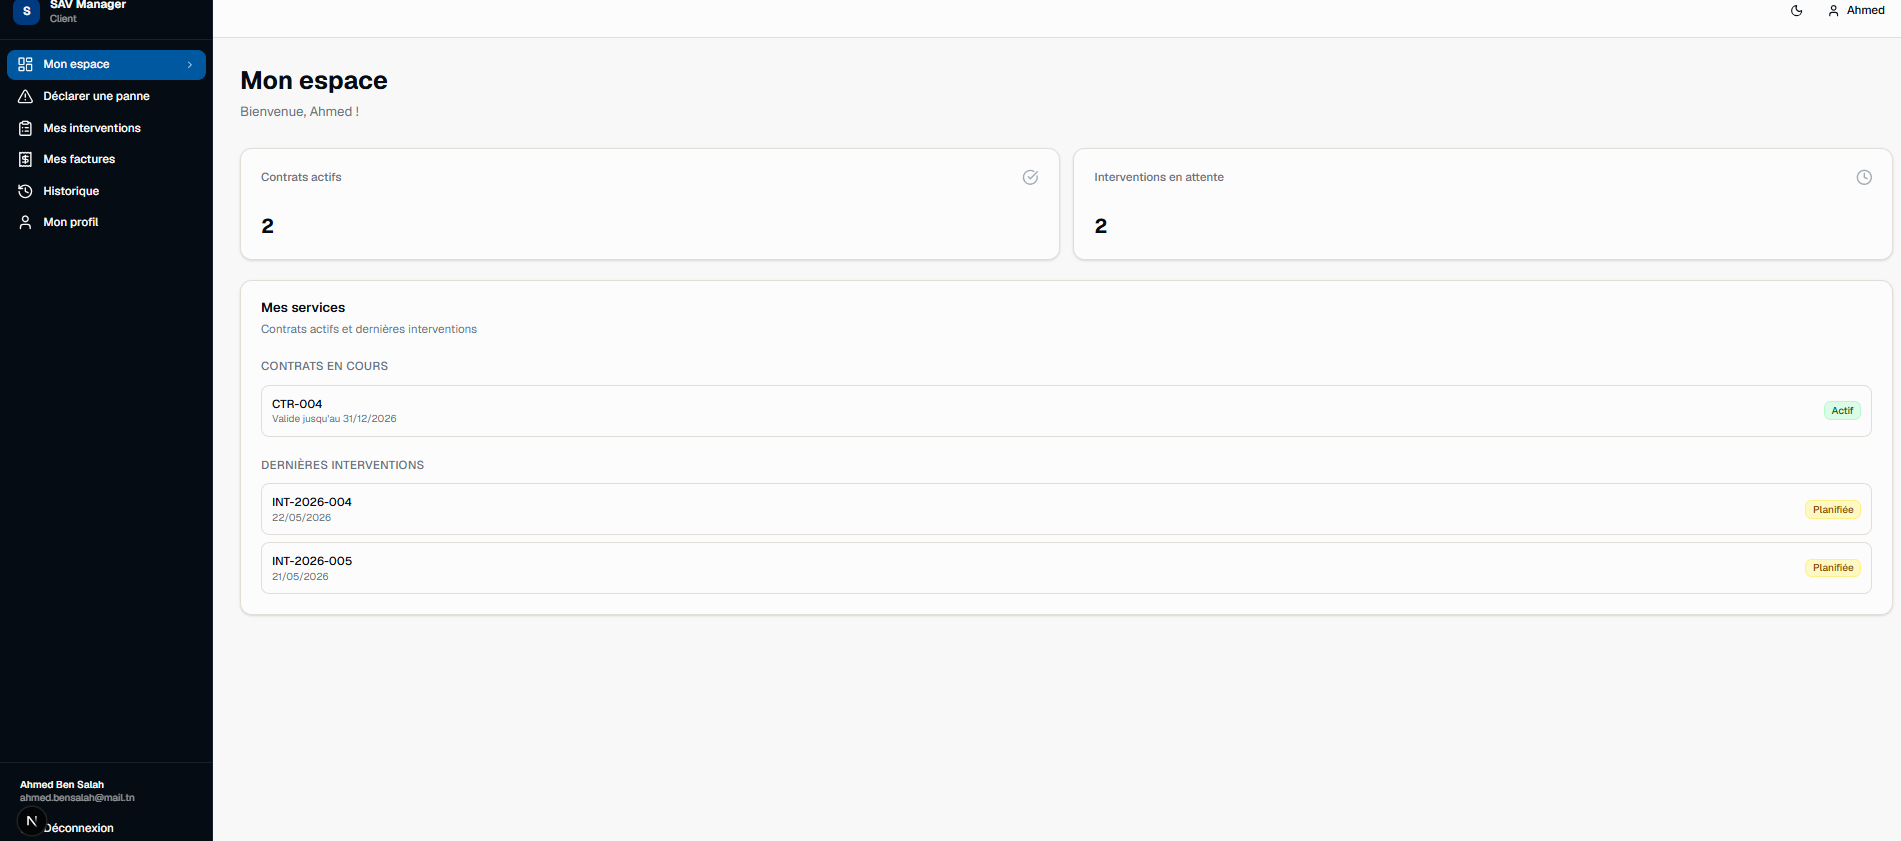
\includegraphics[width=0.74\textwidth]{Figures/Chapitre5/dashboardclientpart.png}
    \caption{Capture d'écran : tableau de bord client}
    \label{fig:ch5:dashboard_client}
\end{figure}

% ─────────────────────────────────────────────────────────────────────────────
\section*{Conclusion}

Ce sprint a permis de finaliser le système SAV avec les fonctionnalités de pilotage : génération
des factures selon les règles d'éligibilité strictes (curative + réalisée + hors contrat), calcul
automatique de la TVA à 19\,\% en dinar tunisien, marquage des factures payées, et des tableaux de
bord différenciés pour l'administrateur, le technicien et le client.
